\documentclass[../main.tex]{subfiles}
\graphicspath{{\subfix{../media/}}}


\begin{document}
	\begin{figure}[h]
		\centering
	    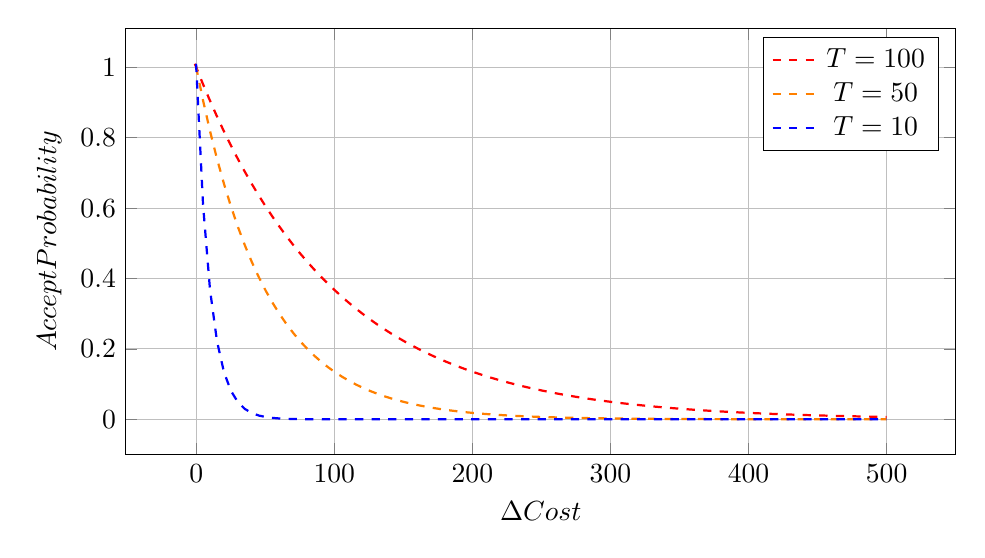
\begin{tikzpicture}
	        \begin{axis}[
	            xlabel = $\Delta \text{Cost}$,
	            ylabel = $\text{Accept Probability}$,
			  	width=\linewidth,
			  	height=7cm,
			  	grid=both,
	            declare function={
	                l0(\cost) = exp(-\cost/100);
	                l1(\cost) = exp(-\cost/10);
	            }
	        ]
	            
	            % Bases Functions
	            \addplot[thick, dashed, red, domain=-1:500, samples=100] {exp(-\x/100)};
	            \addplot[thick, dashed, orange, domain=-0.1:500, samples=100] {exp(-\x/50)};
	            \addplot[thick, dashed, blue, domain=-0.1:500, samples=100] {exp(-\x/10)};
					            
				\legend{$T=100$ , $T=50$, $T=10$}

	        \end{axis}
	    \end{tikzpicture}
	    \caption{Simulated Annealing Temperature }
	\end{figure}


	\SetKwComment{Comment}{/* }{ */}

	\begin{algorithm}
		\caption{Simulated Annealing Algorithm}\label{alg:two}
		\KwData{$T_i, \, x_i $}
		\KwResult{$x_{n} \gets \text{last solution candidate}$}\vspace{5pt}
		$T_0 \gets \text{initial temperature of cooling schedule}$\;
		$x_0 \gets \text{starting solution candidate}$\;\vspace{5pt}

		\For{$i \in \lbrace 0, \dots, n\rbrace$}{
		  $x_\text{neighbor} \gets \text{randomly sample a neighbor from } x_i \text{ neighborhood}$\;
		  $\Delta \, cost \gets \text{compute cost difference between } x_\text{neighbor} \text{ and } x_i$\;\vspace{5pt}
		  \uIf{$\text{cost}(x_\text{neighbor}) \text{ is better than } \text{cost}(x_i)$}{
		    \textbf{Accept} $x_{i+1} \gets x_i$\;\vspace{5pt}
		  }
		  \uElseIf{$\text{cost}(x_\text{neighbor}) \text{ is worse than } \text{cost}(x_i)$}{\vspace{3pt}
		  	\eIf{\text{probability} $e^{-\Delta cost \,/\,T_i}$}{ 
		  		\textbf{Accept} $x_{i+1} \gets x_i$\;\vspace{5pt} 
		  	}
		  	{
		      	\textbf{Reject} \text{Do nothing};\vspace{5pt}
		  	}
		  }
		  }
	\end{algorithm}


\end{document}